%% The shared workspace: several sessions of ONE account, on testbeds that
%% cannot reach each other, agreeing through the one filesystem they all mount.
%% Arrows are DATA FLOW: wiring flows out of the workspace to every session;
%% records and edits flow into it. Labels sit mid-gap with opaque backgrounds.
\documentclass[tikz,border=4pt]{standalone}
\usepackage{xcolor}
%% Shared look for the UnionLabs system figures. \input by each fig-*.tex so a
%% colour or a corner radius is changed in one place.
\usetikzlibrary{positioning,arrows.meta,fit,backgrounds,calc}

\definecolor{uCode}{HTML}{1F6F5C}     % the experimenter's own code
\definecolor{uApi}{HTML}{6B4BA8}      % the contract / ARQ layer
\definecolor{uPhy}{HTML}{2E5E9E}      % transports / DSP
\definecolor{uRadio}{HTML}{B4700F}    % hardware
\definecolor{uShare}{HTML}{8A2E4D}    % the shared workspace

\tikzset{
  blk/.style={draw, rounded corners=2pt, align=center, font=\small,
              minimum height=8mm, inner sep=3pt, fill=black!2},
  code/.style={blk, draw=uCode, thick, fill=uCode!6},
  api/.style={blk, draw=uApi, very thick, fill=uApi!7},
  phy/.style={blk, draw=uPhy, thick, fill=uPhy!6},
  radio/.style={blk, draw=uRadio, thick, fill=uRadio!8},
  share/.style={blk, draw=uShare, thick, fill=uShare!6},
  stage/.style={blk, minimum height=9.5mm, font=\scriptsize, text width=16mm,
                inner sep=2pt},
  flow/.style={-{Latex[length=2mm]}, thick},
  back/.style={-{Latex[length=2mm]}, thick, densely dashed},
  % labels that sit ON an arrow: opaque, so the line never strikes the text
  onarrow/.style={font=\scriptsize\itshape, fill=white, inner sep=1.5pt},
  lbl/.style={font=\scriptsize\itshape, inner sep=1pt},
  note/.style={font=\scriptsize, align=left, inner sep=1pt},
  legend/.style={draw, minimum width=3mm, minimum height=3mm, inner sep=0pt},
}
\newcommand{\mono}[1]{{\ttfamily\footnotesize #1}}
\newcommand{\monos}[1]{{\ttfamily\scriptsize #1}}

\begin{document}
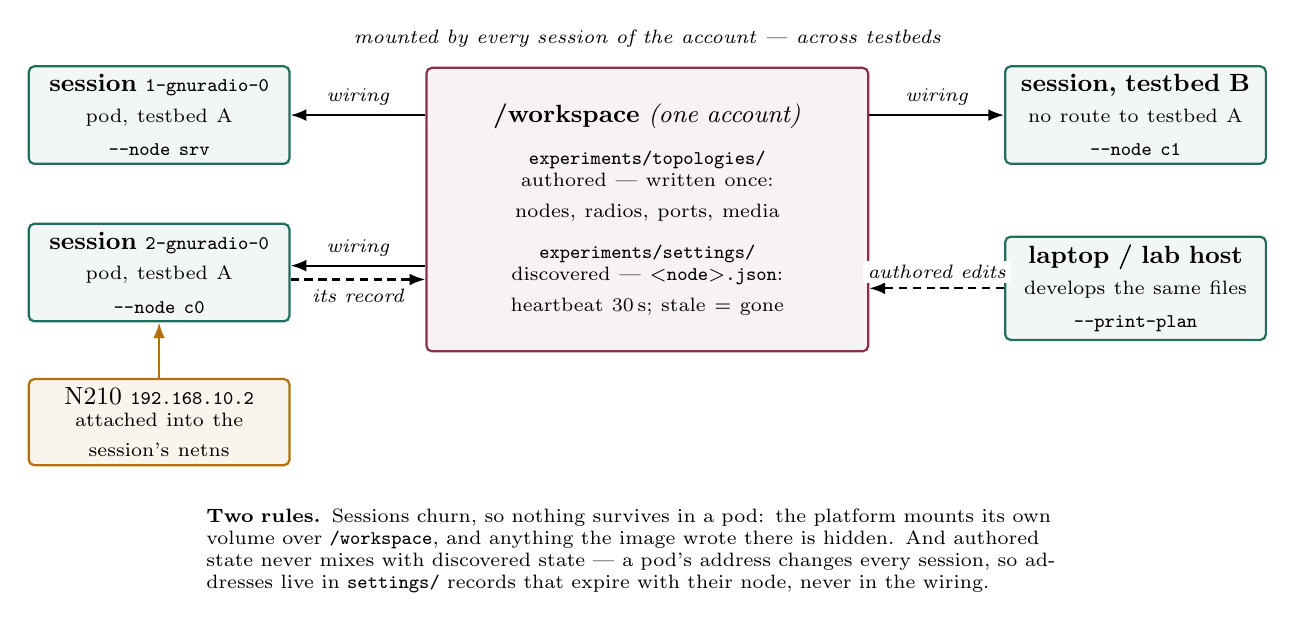
\begin{tikzpicture}[x=1mm, y=1mm]

%% ── the workspace in the middle ──────────────────────────────────────────
\node[share, text width=54mm, minimum height=36mm] (ws) at (0,0)
  {\textbf{/workspace} \emph{(one account)}\\[4pt]
   \monos{experiments/topologies/}\\
   {\scriptsize authored --- written once:\\ nodes, radios, ports, media}\\[4pt]
   \monos{experiments/settings/}\\
   {\scriptsize discovered --- \monos{\textless node\textgreater.json}:\\ heartbeat 30\,s; stale $=$ gone}};
\node[lbl, above=2mm of ws.north] {mounted by every session of the account --- across testbeds};

%% ── testbed A, left ──────────────────────────────────────────────────────
\node[code, text width=31mm] (s1) at (-62,12)
  {\textbf{session} \monos{1-gnuradio-0}\\{\scriptsize pod, testbed A}\\[1pt]
   \monos{--node srv}};
\node[code, text width=31mm] (s2) at (-62,-8)
  {\textbf{session} \monos{2-gnuradio-0}\\{\scriptsize pod, testbed A}\\[1pt]
   \monos{--node c0}};
\node[radio, text width=31mm] (n210) at (-62,-27)
  {N210 \monos{192.168.10.2}\\{\scriptsize attached into the\\ session's netns}};

%% ── elsewhere, right ─────────────────────────────────────────────────────
\node[code, text width=31mm] (s3) at (62,12)
  {\textbf{session, testbed B}\\{\scriptsize no route to testbed A}\\[1pt]
   \monos{--node c1}};
\node[code, text width=31mm] (s4) at (62,-10)
  {\textbf{laptop / lab host}\\{\scriptsize develops the same files}\\[1pt]
   \monos{--print-plan}};

%% ── data flow ────────────────────────────────────────────────────────────
\draw[flow] (ws.west |- s1) -- node[onarrow, above=1.5pt] {wiring} (s1.east);
\draw[flow] ([yshift=2.5]ws.west |- s2) -- node[onarrow, above=1.5pt] {wiring}
            ([yshift=2.5]s2.east);
\draw[back] ([yshift=-2.5]s2.east) -- node[onarrow, below=1.5pt] {its record}
            ([yshift=-2.5]ws.west |- s2);
\draw[flow] (ws.east |- s3) -- node[onarrow, above=1.5pt] {wiring} (s3.west);
\draw[back] (s4.west) -- node[onarrow, above=1.5pt] {authored edits}
            (ws.east |- s4);
\draw[flow, draw=uRadio] (n210.north) -- (s2.south);

%% ── the two rules ────────────────────────────────────────────────────────
\node[note, text width=112mm, anchor=north]
  at ([yshift=-5mm]current bounding box.south)
  {\textbf{Two rules.} Sessions churn, so nothing survives in a pod: the
   platform mounts its own volume over \monos{/workspace}, and anything the
   image wrote there is hidden. And authored state never mixes with discovered
   state --- a pod's address changes every session, so addresses live in
   \monos{settings/} records that expire with their node, never in the wiring.};

\end{tikzpicture}
\end{document}
